\documentclass[letterpaper,12pt,twoside]{maths}
\usepackage[utf8]{inputenc}
\usepackage[english]{babel}
\usepackage{fancyhdr}
\usepackage[margin=1in]{geometry}
\usepackage{graphicx}
\usepackage{amsmath} 
\usepackage{mathtools}
\usepackage[mathscr]{euscript} 
%\newcommand*{\ms}[1]{\ensuremath{\mathscr{#1}}}
\usepackage{lmodern} % math, rm, ss, tt
\usepackage[T1]{fontenc}
     
\pagestyle{fancy} 
\fancyhf{}
\chead{Section 3} 
\rhead{Spring 2019}   
\lhead{\vspace{3mm} Math 147 Topology}
\rfoot{Page \thepage} 
\linespread{1.3}
   

\renewcommand{\headrulewidth}{2pt}
\renewcommand{\footrulewidth}{1pt}

\graphicspath{ {./figures_theorems_sect_3/} } 

% info for header block in upper right hand corner
\begin{document}
\section*{3.1 Topological Spaces: Fundamentals}  

\begin{problem}[Theorem 3.1.] Let $\{U_i\}_{i=1}^n$ be a finite
 collection of open  sets in a topological space $(X, \mathscr{T})$.
 Then $\cap_{i=1}^n U_i$ is open.
\end{problem}                 

\begin{proof}
    We'll do this with mathematical induction. Let the
    base case be $n = 1$. Then observe that
    \[
      \bigcap\limits_{i=1}^1U_i = U_i  
    \]
    which is open by hypothesis. 
    \\
    \\
    Now we perform the inductive step. Suppose the statement holds for
    the integer $n \ge 1$. Let $V$ be any open set. Then 
    \[
      \left(\bigcap\limits_{i = 1}^n U_i \right) \cap V  
    \] 
    is the intersection of two open sets, (by hypothesis, both 
    $\bigcap\limits_{i = 1}^n U_i$ and $V$) are open, and so by     
    condition (3) of a topology the intersection of $n+1$ open sets is
    open. As the statement holds for $n+1$, we have by mathematical
    induction that it holds for all $n \in \mathbb{N}$.  
\end{proof}

\noindent
\begin{exercise}[Exercise 3.2]
    Why does your proof not prove the false
    statement that the infinite intersection of open sets is necessarily
    open? 
\end{exercise}
 
\begin{solution}
    The answer to this lies in the fact that a proposition which is proven
to be true by mathematical induction does not imply 
that the proposition is
true for an infinite number of steps. Thus the proof does not prove
the false statement that infinite intersections are open.
\end{solution}


\begin{problem}[Theorem 3.3] A set $U$ is open in a topological space
    $(X, \mathscr{T})$ if and only if for every point $x \in U$, there
    exists an open set $U_x$ such that $x \in U_x \subset U$.
\end{problem}

\begin{proof}
    We'll prove one direction at a time. Suppose that
    we have a set $U$ such that, for every $x \in U$, there exists an
    open set $U_x$ such that $x \in U_x \subset U$. Now suppose we
    take the (possibly uncountable) union of each of these open sets
    $U_x$. Observe that, since for each $x$ we have $U_x \subset U$,
    \[
        \bigcup\limits_{x \in U} U_x = U.
    \] 
    However by condition (4) in the
    definition of a topology, we know that this ought to be inside our
    topology $\mathscr{T}$, which proves that $U$ must be an open set.
    \\
    \\
    Now we prove the other direction. Consider an arbitrary point $x
    \in U$, where $U$ is an open set in our topology $\mathscr{T}$.
    Let $V$ be any neighborhood about $x$. Observe that $U \cap V$ is
    an open set such that $x \in U_x \subset U.$ Thus we have found
    our open neighborhood $U_x$, proving the other direction of the
    theorem. Thus the theorem itself is true. 

\end{proof}

\begin{exercise}[Exercise 3.4]
Verify that $\mathscr{T}_{\text{std}}$ is a
topology on $\mathbb{R}^n$; in other words, it satisfies the four
conditions of the definition of a topology. 
\end{exercise}

\begin{solution}
    \begin{enumerate}
        \item Observe that the first condition is satisfied, namely that $\emptyset
        \in \mathscr{T}_{\text{std}}.$ This is because the condition to be in
        $\mathscr{T}_{\text{std}}$ is vacuously true for the empty set because
        there are no elements in the empty set. 
    
        \item Now consider the set $\mathbb{R}^n$ itself. 
        For any point $p \in
        \mathbb{R}^n$, $B(p, \epsilon) \subset \mathbb{R}^n$ for
        any $\epsilon > 0$. Thus by the definition of
        $\mathscr{T}_{\text{std}}$,
        we have that $\mathbb{R}^n \in
        \mathscr{T}_{\text{std}}$. Condition two is satisfied.
    
        \item Now consider two elements $U, V \in \mathscr{T}_{\text{std}}$. Suppose
        that $U \cap V \ne \emptyset$; otherwise it is trivial. So consider an
        element $p \in U \cap  V.$ Then there exists two balls $B(p,
        \epsilon_1) \subset U$ and $B(p, \epsilon_2) \subset V$ where
        $\epsilon_1, \epsilon_2 > 0$. On this subset, observe that $B(p,
        \text{min}\{\epsilon_1, \epsilon_2\}) \subset U\cap V.$ First note
        that we can certainly conclude that $B(p,\epsilon_1) \cap B(p,
        \epsilon_2) \subset U \cap V.$ Now because $B(p,\epsilon_1)$ and $B(p,
        \epsilon_2)$ are balls about the same point, we know that
        $B(p,\epsilon_1) \cap B(p, \epsilon_2) = B(p, \text{min}\{\epsilon_1,
        \epsilon_2\})$, so that we may conclude $U\cap V \in
        \mathscr{T}_{\text{std}}$. Thus condition three is satisfied. 
        
        \item  Finally, we'll verify the fourth condition. Consider 
        $\{U_{\alpha} \}_{\alpha \in \lambda}$ where
        $\lambda$ is an arbitrary index set such that $U_\alpha \in
        \mathscr{T}_{\text{std}}$. Thus for each $\alpha \in \lambda$, and for
        every point $p \in U_\alpha$, there exists an open ball $B(p,
        \epsilon_{(\alpha, p)}) \subset U_\alpha$ such that
        $\epsilon_{(\alpha, p)} > 0$.
        Next, suppose $p \in 
    \bigcup\limits_{\alpha \in
    \lambda} U_\alpha$. Then $p \in U_\alpha$ for at least one $\alpha \in
        \lambda$, so that $B(p, \epsilon(\alpha, p)) \subset U_\alpha$.
        Since $p$ was arbitrary in $\bigcup\limits_{\alpha \in
        \lambda} U_\alpha$, we have that $\bigcup\limits_{\alpha \in
        \lambda} U_\alpha \in \mathscr{T}_{\text{std}}$ as desired. 
    \end{enumerate}
\end{solution}

\begin{exercise}[3.5]
    Verify that the discrete, indiscrete, finite
    complement and countable complement topologies are indeed topologies
    on any set $X$. 
\end{exercise} 

\begin{solution}
    We can verify that the finite complement topology $\mathscr{T}$ on a
set $X$ is a true topology on $X$ as follows. 
\begin{enumerate}
    \item First observe that in
    the definition of the topology $\emptyset$ is said to be in the
    topology so the first condition of a topology is satisfied. 

    \item Next we can verify the second property of topologies. It is obvious
    that $X \in \mathscr{T}$. This is because $X - X = \emptyset$ which is
    itself a finite set. 
    
    \item Now if $U, V \in \mathscr{T}$, then $X - U$ and $X - V$ are both
    finite sets. Therefore, we can conclude that $(X - U) \cup (X - V)$ is
    a finite set. However, by De Morgan's laws, $(X - U) \cup (X - V) = X
    - (U \cap V)$, and because this is a finite set, we must conclude that
    $U \cap V \in \mathscr{T}$. Thus the third property of a topology is
    verified. 

    \item Finally, we verify the last property in the defintion of a topology.
    Suppose $U_\beta \in
    \mathscr{T}$ for all $\beta \in \lambda.$ Now observe that for some $\beta \in
    \lambda$, $X - U_\beta$ is a finite set. But observe that $X -
    \cup_{\alpha \in \lambda}U_\alpha \subset X - U_\beta$, so that $X -
    \cup_{\alpha \in \lambda}U_\alpha$ must also be a finite set. Thus we
    see that $\cup_{\alpha \in \lambda}U_\alpha \in \mathscr{T}$, proving
    the last property which verifies that $\mathscr{T}$ is a true topology
    on $X$. 
\end{enumerate}

\end{solution}

\begin{exercise}[Exercise 3.7]
    Give an example of a topological space and a
    collection of open sets in that topological space that show that
    infinite intersections of open sets need not be open 
\end{exercise}

\begin{solution}
    We can borrow the example I provided in Exercise 3.2. 
    Consider the standard
    topology on $\mathbb{R}$ and observe that $\displaystyle \bigcap_{n=1}^\infty
    \left(-\frac{1}{n}, \frac{1}{n}\right) = \{0\}$. $\{0\}$ isn't an open set under
    the standard topology, so that this example shows that countable
    intersections of open sets may not be open. 
\end{solution}


\begin{exercise}[Exercise 3.8]
    Let $X = \mathbb{R}$ and $A = (1,2)$. Verify
    that 0 is a limit point $A$ in the indiscrete topology and the finite
    complement topology, but not in the standard topology nor the discrete
    topology of $\mathbb{R}.$ 
\end{exercise}

\begin{solution}
    In the indiscrete topology, the only possible set that can contain 0
is simply $\mathbb{R}$ itself, for which $\mathbb{R} \cap (1,2) \ne
\emptyset$. Thus 0 must be a limit point of $(1,2)$. \\
\\
In the finite complement topology on $\mathbb{R}$, the open sets which
contain 0 must be sets $U$ such that $\mathbb{R} - U$ is finite and $0
\in U$. Now since $\mathbb{R} - U$ must be finite while (1,2) is obviously
uncountable, it will never be the case that $(1, 2) \subset (\mathbb{R}
- U)$. Therefore, 
$(U - \{0\}) \cap (1,2)) \ne \emptyset$ for all $U$ in the finite
complement topology. Thus 0 must be a limit point
of $(1,2)$ in this toplogy. \\
\\
Now 0 is obviously not a limit point of (1,2) in the standard
topology. This can be demonstrated by simply constructing a ball such
as $B(0, 1/2)$ (a ball about $0$ of radius 1/2) to show the existence
of one open set $U$ about $0$ such that $U \cap A = \emptyset$. Hence,
0 is not a limit point of (1,2).\\
\\
0 is also not a limit point of (1,2) in the discrete topology. For
example, consider the open set $\{0\}$ which contains 0 but obviously
$\{0\} \cap (1,2) = \emptyset.$ Again, by theorem 3.9, we can see that
0 is not a limit point of (1,2) in this topology.

\end{solution}

\begin{problem}[Theorem 3.9] Suppose $p \notin A$ in a topological
space $(X, \mathscr{T})$. Then $p$ is not a limit point of $A$ if and
only if there exists a neighborhood $U$ of $p$ such that $U \cap A =
\emptyset$.
\end{problem}

\begin{proof}
    First suppose that there exists a exists a
    neighborhood $U$ of $p$ such that $U \cap A = \emptyset.$ Then by
    definition, this cannot be a limit point, since the requirement to
    be a limit point is
    that every neighborhood of $p$ must contain a point $q \ne p$
    where $q \in A$. Clearly we we see that this condition cannot be
    satisfied, so $p$ cannot be a limit point. \\
    \\
    We can prove the other direction by supposing now that $p$ is not
    a limit point of $U$. Since $p$ is not a limit point, we know by
    definition that there exists at least one neighborhood $U$ of $p$
    such that $(U - \{p\}) \cap A = \emptyset$. Since we are given
    that $p \notin A$, we can 
    further state that $U \cap A = \emptyset$. 
    Thus we have found our set $U$ of $p$
    such that $U \cap A = \emptyset$, which proves the theorem.    
\end{proof}


\begin{exercise}[Exercise 3.10]
    If $p$ is an isolated point of a set $A$ in a topological space $X$,
    then there exists an open set $U$ such that $U \cap A = \{p\}$.    
\end{exercise}

\begin{solution}
Since $p$ is an isolated point, we know that $p$ is not a limit point
of $A$. By definition of a limit point, this means that there exists
at least one open set $U$ containing $p$ such that $(U-\{p\}) \cap A =
\emptyset$. Since $p \in A$ and $p \in U$,
we can then state that $U \cap A =
\{p\}$, as desired. Thus such a $U$ described in the problem statement
exists.
\end{solution}

\begin{exercise}[Exercise 3.11]
Give examples of sets $A$ in various topological spaces $(X,
\mathscr{T})$ with\\
1. A limit point of $A$ that is an element $A$;\\
2. A limit point of $A$ that is not an element of $A$;\\
3. An isolated point of $A$;\\
4. A point not in $A$ that is not a limit point of $A$; 
\end{exercise}

\begin{solution}
\begin{enumerate}
    \item Consider the standard topology $\mathscr{T}_{\text{std}}$ on
    $\mathbb{R}$. For any interval $(a,b) \subset \mathbb{R}$ where $a < b$ we have
    that any point $x \in (a,b)$ is a limit point since, for any
    neighborhood $U$ about $x$, $(U - \{x\}) \cap (a,b) \ne
    \emptyset$.
    since for any
    neighborhood of $x$ there exists a ball $B(x, \epsilon)$ such that
    $B(x, \epsilon) \subset U$.
    
    \item For any interval $(a,b)$ as defined in (1.), we have that $a$ and
    $b$ are both limit points of the interval. This is because any open
    set about these two points will always include other points in
    $(a,b)$. For example, if we construct a ball $B(a, \epsilon)$ (a
    neighborhood about $a$ with radius $\epsilon$) then any point in the
    interval $(a, a + \epsilon) \subset (a,b)$ can be found within the
    ball, so that $B(p, \epsilon) \cap (a, b) \ne \emptyset$. 
    This analogously holds for $b$, so
    for any open set $U$ about $a$ or $b$, we have that $(U -
    \{a\}) \cap (a,b) \ne \emptyset$ or $(U - \{b\}) \cap (a,b) \ne
    \emptyset$, so that $a,b$ are both limit points of $(a,b)$.

    \item Let $x \in \mathbb{R}$ such that $x \notin (a,b)$, and observe
    that $x$ is an isolated point of the set $\{x\} \cup (a,b)$. In this
    example, $x$ is quite literally an isolated point!

    \item Any point $x
    \notin (a,b)$ is a point that is not in $(a,b)$ and is not a limit
    point of $(a,b)$. 
\end{enumerate} 
\end{solution}
       
\begin{problem}[Theorem 3.13] For any topological space $(X,
    \mathscr{T})$ and $A \subset X$, $\overline{A}$ is closed. That
    is, for any set $A$ in a topological space,
    $\overline{\overline{A}} = \overline{A}$, 
\end{problem}

\begin{proof}                    
    To prove this, let $p$ be a limit point of $\overline{A}$. Then
    for every open set $U$ which contains $p$, we know that 
    \[
        (U-\{p\})\cap \overline{A} \ne \emptyset.
    \] 
    Thus for each $U$ there exists a point $q \in
    \overline{A}$ such that $q \in U$ and $q \ne p$.
    \\
    If $q \in A$, then we see
    that 
    \[
        (U-\{p\}) \cap A \ne \emptyset.
    \] 
    If $q$ is a limit point of
    $A$, then every open set containing $q$ must intersect
    with $A$. Since $U- \{p\}$ is an open set containing $q$, we
    can also conclude that the set $U - \{p\}$ must
    itself intersect with $A$. Either way, we have shown that for
    every open set $U$ which contains $p$, $(U - \{p\}) \cap A \ne
    \emptyset$. In other words, if $p$ is a limit point of
    $\overline{A}$ then $p \in \overline{A}$, so
    $\overline{\overline{A}} \subset \overline{A}$.
    Since it is trivial that $\overline{A} \subset
    \overline{\overline{A}},$
    we must have that $\overline{\overline{A}} = \overline{A}$ 
    as desired.
\end{proof}


\begin{problem}[Theorem 3.14] Let $(X, \mathscr{T})$ be a topological
    space. Then the set $A$ is closed if and only if $X-A$ is open. 
\end{problem}

\begin{proof}
    First we begin with the forward direction by supposing $A$ is a
    closed set. Then $A$ must contain all of its limit points, so $X -
    A$ contains no limit points of $A$. \\By Theorem 3.9, we can
    conclude that for all $p \in X-A$, there exists an open set $U$
    about $p$ such that $U \cap A = \emptyset \implies p \in U 
    \subset X - A$. Since this holds for all $p \in X - A$,
    by Theorem 3.3 this means
    that $X - A$ is an open set, which is what we set out to show. \\
    \\
    Now we prove the other direction, and suppose that $X - A$ is an
    open set. Since
    $X - A$ is open, we know that for every point $q \in X - A$, there
    exists an open set $U$ of $q$ such that $U \subset X - A$ and
    therefore $U \cap A = \emptyset$. Thus we see that none of the $q
    \in X -A$ could possibly be a limit point of $A$ since every point
    of $X - A$ violates the definition of a limit point of $A$. 
    Thus all the limit
    points of $A$ must be in $A$, so that $A$ is closed. With both
    directions proven, the theorem is itself proved. 

\end{proof}

\begin{problem}[Theorem 3.15] Let $(X, \mathscr{T})$ be a topological
    space, and let $U$ be an open set and $A$ be a closed subset of
    $X$. Then the set $U - A$ is open and $A - U$ is closed.
\end{problem}

\begin{proof}
    We can show that $U - A$ is open as follows. Since $A$ is closed,
    we know that $X - A$ must be an open set by Theorem 3.14. Now $U - A = U \cap (X -
    A)$, so $U - A$ is the intersection of two open sets and hence is
    itself an open set, which is what we set out to show.\\
    \\
    Next, observe that $A - U$ = $A \cap (X - U)$. Thus $A - U$ 
    is the intersection of two closed sets, which implies that $A - U$
    is itself closed, as desired.
\end{proof}
\begin{figure}[h!]
    \centering
    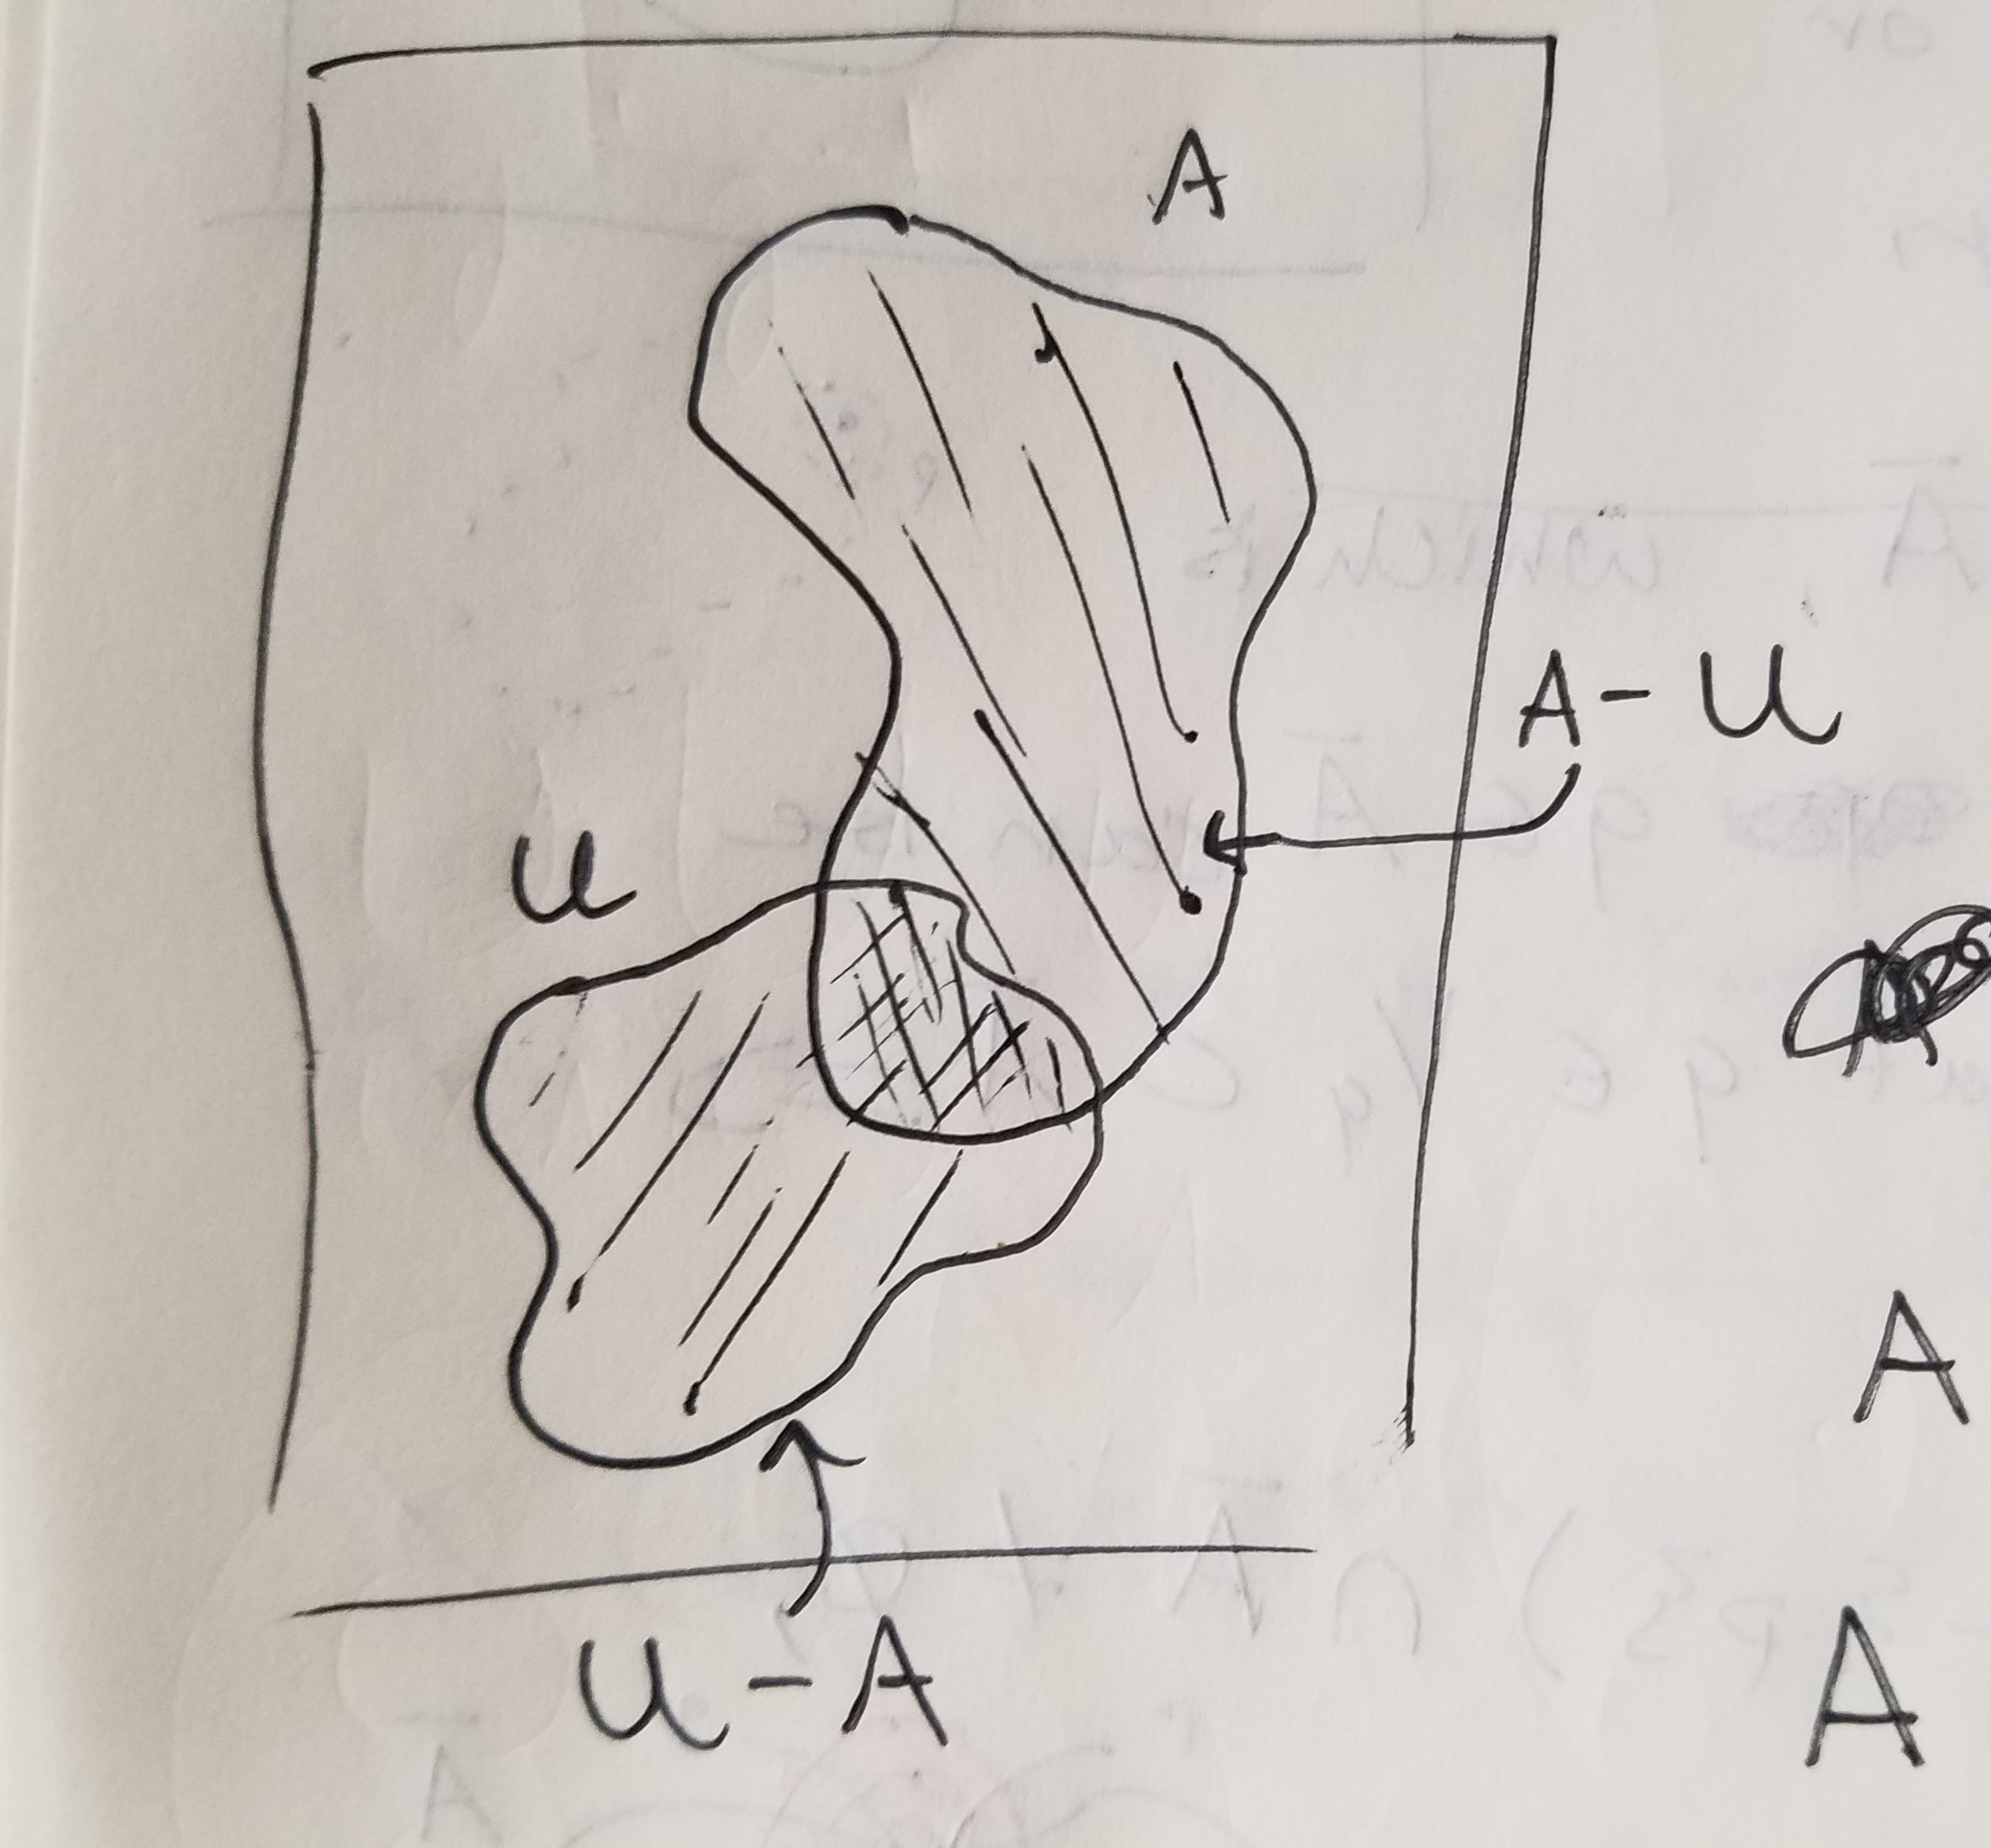
\includegraphics[width=0.6\textwidth]{sketch_theorem_3_15_2.jpg}
    \caption{Two arbitrary sets $U$ and $A$ are drawn as well as the
    sets $A-U$ and $U-A$.}
\end{figure}

\begin{problem}[Theorem 3.16] Let $(X, \mathscr{T})$ be a topological
    space. Then:\\
    \textit{i}) $\emptyset$ is closed.\\
    \textit{ii}) $X$ is closed.\\
    \textit{iii}) The union of finitely many closed sets is closed.\\
    \textit{iv}) Let $\{A_{\alpha}\}_{\alpha \in \lambda}$ be a
    collection of closed subsets in $(X, \mathscr{T})$. Then
    $\cap_{\alpha \in \lambda} A_\alpha$ is closed.
\end{problem}

\begin{proof}
    We can first prove (\textit{i}) by observing that, since the empty
    set contains no elements, it is vacuousely true that it contains
    all of its limit points. Thus $\emptyset$ is a closed set. \\
    \\
    To prove (\textit{ii}), observe that $X$, 
    the entire space, must contain all of its limit points. Thus
    $X$ is a closed set. \\
    \\
    For (\textit{iii}), let $p$ be a limit point of $\bigcup\limits_{i = 1}^n
    A_i$. Then for at least for every neighborhood $U$ of $p$ we
    have that $(U - \{p\}) \cap \bigcup\limits_{i = 1}^n A_i \ne \emptyset$ so that 
    $(U - \{p\})\cap A_i \ne \emptyset$ for at least one $A_i$ 
    in of $\{A_i\}_{i = 1}^n$. Thus all the limit points of
    $\bigcup\limits_{i = 1}^n
    A_i$ are simply limit points of the sets in $\{A_i\}_{i = 1}^n$.
    Thus $\bigcup\limits_{i = 1}^n A_i$ contains all of its limit points so
    it is a closed set.
    \\
    \\
    demorgans laws \\
    \\
    To prove (\textit{iv}), consider an arbitrary collection of closed
    sets $\{A_\alpha\}_{\alpha \in \lambda}$, where $\lambda$ is an
    arbitrary index. Observe that by DeMorgan's Laws
    \[
        \left(\bigcap\limits_{\alpha \in \lambda} A_\alpha\right)^c
        = \bigcup\limits_{\alpha \in \lambda} A_\alpha^c.
    \]
    Observe that each $A_\alpha^c$ is an open set by Theorem 3.14, and
    because the arbitrary union of open sets is open, we can then
    conclude that $\bigcup\limits_{\alpha \in \lambda} A_\alpha^c$ 
    is an open set. Since $\left(\bigcap\limits_{\alpha \in \lambda} A_\alpha\right)^c
    = \bigcup\limits_{\alpha \in \lambda} A_\alpha^c$, 
    Theorem 3.14 tell us
    that $\bigcap\limits_{\alpha \in \lambda} A_\alpha$ is a closed
    set, as desired.
\end{proof}


\noindent
\begin{exercise}[Exercise 3.17] Give an example to show that the union of
infinitely many closed sets in a topological space may be a set that
is not closed.
\end{exercise}

\begin{solution}
On the standard topology of $\mathbb{R}$, we can take the example that
$\cup_{n=1}^\infty [-n, n]$. The resulting set is no longer a closed
set, since for every point in the resulting set we can construct a
neighborhood about every point such that the neighborhood is entirely
contained in the set. 
\end{solution}

\begin{exercise}[Exercise 3.18]
    Give examples of topological spaces and sets in
    them that:\\
1. are closed, but not open;\\
2. are open, but not closed;\\
3. are both open and closed; \\
4. are neither open nor closed. 
\end{exercise}

\begin{solution}
    \begin{enumerate}
        \item In the standard topology on $\mathbb{R}$, closed sets are
        definitely not open sets.
    
        \item Again, in the standard topology, open sets are not the same thing
        as closed sets. We can also use the example of the discrete topology,
        since every subset is considered to be an open set. None of the sets
        are closed.
    
        \item In the indiscrete topology, every set is both open and closed since
        each set simultaneously contains all of its limit points and every
        point in each set can be contained in a ball which is a subset of the
        respective set.
    
        \item Consider the finite complement topology on $\mathbb{R}$. The set
        $\mathbb{Z}$ is not open or closed in this topology. 
    \end{enumerate}
\end{solution}

\begin{exercise}[Exercise 3.19]
State whether each of the following sets are
open, closed, both, or niether.\\
1. In $\mathbb{Z}$ with the finite complement topology: $\{0, 1, 2\},
\{\text{prime numbers}\}, \{n : |n| \ge 10\}$\\
2. In $\mathbb{R}$ with the standard topology: (0,1), (0,1], [0,1],
$\{0,1\}$, $\{\frac{1}{n} : n \in \mathbb{N}\}$.\\
3. In $\mathbb{R}^2$ with the standard topology: $\{(x,y) : x^2 + y^2
= 1\}, \{(x,y) : x^2 + y^2 > 1\}, \{(x,y) : x^2 + y^2 \ge 1\}.$ 
\end{exercise}

\begin{solution}
    \begin{enumerate}
        \item The set $\{0, 1, 2\}$ is not an open set. Furthermore, it cannot be
        a closed set since it has no limit points (or does this vacuousely
        prove that it is a closed set?). 
        The prime numbers are also not an open set. 
        The set $\{n : |n| \ge 10\}$ is definitely an open set since
        $\mathbb{Z} - \{n : |n| \ge 10\} = \{-9, -8, \dots, 8, 9\}$
    
        \item (0,1) is an open set in this topology since every point $x \in
        (0,1)$ can be contained in a neighborhood which is a subset of
        $(0,1)$.
        \\
        \\
        (0, 1] is neither an open or closed since, since it doesn't contain
        all of its limit points and not every point can be in a neighborhood
        entirely contained in the set.
        \\
        \\
        $[0,1]$ is a closed set since it contains all of its limit points.\\ 
        $\{0, 1\}$ is not an open set because not every neighborhood
        containing either 0 or 1 will be entirely contained in the set. It is
        also not a closed set since it doesn't have any limit points (or does
        this imply that it can be a closed set?). 
        \\
        \\
        Finally, $\{\frac{1}{n} : n \in \mathbb{N}\}$ is not a closed set
        because it doesn't contain its one limit point, 0. It is also not an
        open set because not every neighborhood of every point of the set can
        be entirely contained in the set.
        
        \item The set $\{(x,y) : x^2 + y^2 = 1\}$ cannot be open since not every
        open set about an element of the set will be entirely contained in the
        set. It is however open because it contains all of its limit
        points.
        \\
        \\
        The set $\{(x,y) : x^2 + y^2 > 1\}$ is open because every point can be
        contained by an open set which is in turn contained in the entire set.
        It is not closed because it does not contain its limit points.
        \\
        \\
        Finally, the set $\{(x,y) : x^2 + y^2 \ge 1\}$ is closed because it
        contains all of its limit points which lie on the circle. 
    
    \end{enumerate}
\end{solution}

\begin{problem}[Theorem 3.20] For any set $A$ in a topological space
    $X$, the closure of $A$ equals the intersection of all closed sets
    containing $A$, that is,
    $$
    \overline{A} = \bigcap\limits_{A \subset B, B \in \mathscr{C}} B
    $$
    where $\mathscr{C}$ is the collection of all closed sets in $X$.
\end{problem}

\begin{proof}
    Observe that $\overline{A}$ is a closed set which contains $A$ so
    that 
    $\overline{A} \in \mathscr{B}$. Thus we'll have that
    $\bigcap\limits_{A
    \subset B, B \in \mathscr{C}} B \subset \overline{A}$. Next
    observe that for all $B \in \mathscr{C}$, $\overline{A} \subset
    B$. This is because $\overline{A}$ 
    is the smallest closed set which contains $A$.
    We can argue this by noting that if we delete any
    point from $\overline{A}$, we'd either delete a point of $A$
    and we'd no longer contain $A$, or we'd delete a limit point of
    $A$ and our set would no longer be closed. Hence $\overline{A}$ is
    the smallest closed set containing $A$.\\
    \\
    Since $\overline{A} \subset B$ for all $B \in \mathscr{C}$, we can
    then state that $\overline{A} \subset \bigcap\limits_{A \subset B, B \in
    \mathscr{C}} B$. Since we already showed that $\cap_{A \subset B,
    B \in \mathscr{C}} B \subset \overline{A}$, this becomes
    sufficient to prove that $\overline{A} = \bigcap\limits_{A \subset B, B \in
    \mathscr{C}} B$.

\end{proof}

\begin{exercise}[Exercise 3.21]
    Pick several different subsets of $\mathbb{R}$
and find their closures in:
\begin{itemize}
    \item[1.] the discrete topology;
    \item[2.] the indiscrete topology;
    \item[3.] the finite complement topology; 
    \item[4.] the standard topology. 
\end{itemize}
\end{exercise}

\begin{solution}
    \begin{itemize}
        \item[1.]Consider the $(0,1)$. Then in the discrete topology, we know that
        the closure is just the set itself, because every set in the discrete
        topology is closed.
    
        \item[2.] In the indiscrete topology. the closure of the set is all of
        $\mathbb{R}$, since every point of $\mathbb{R}$ is a limit point of
        $(0,1)$.
    
        \item[3.] In this case, every point of $\mathbb{R}$ is also a limit point to
        the finite complement topology, since every open set will always
        contain points in $(0, 1)$ because it is uncountably infinite.
    
        \item[4.] In the standard topology, $[0,1]$ would be the closure of the set
        since $0, 1$ are the limit points of the set. 
        \end{itemize}
\end{solution}

\begin{problem}[Theorem 3.22.] Let $A$ and $B$ be subsets of a
    topological space $X$. Then
    \begin{itemize}
        \item[1.] $A \subset B$ implies $\overline{A} \subset \overline{B}$
        
        \item[2.] $\overline{A \cup B} = \overline{A} \cup \overline{B}.$
    \end{itemize}
\end{problem}

\begin{proof}
    Consider a limit point $p$ of $A$. By definition, for every open
    set $U$ of $p$, we have that $(U - \{p\}) \cap A \ne \emptyset.$
    However, since $B$ contains $A$, we can also state that $(U -
    \{p\}) \cap B \ne \emptyset$, meaining that $p$ must also be a
    limit point of $B$. Thus $\overline{A} \subset \overline{B}.$ 

    Consider limit points $p, q$ of $A, B$ respectively. Then for all
    open sets $U, V$ containing $p, q$ respectively, we'll have that
    $(U - \{p\}) \cap A \ne \emptyset$ and $(V - \{q\}) \cap B \ne
    \emptyset$. Now it is definitely true that for these same open
    sets that $(U - \{p\}) \cap (A \cup B) \ne \emptyset$ and $(V -
    \{q\}) \cap (A\cup B)$, so that both $p$ and $q$ must be limit
    points of $A \cup B$. Thus $\overline{A} \cup \overline{B} \subset
    \overline{A \cup B}.$ 
    
    Now suppose that $r$ is a limit point of
    $\overline{A \cup B}.$ Then this means that for every open set $W$
    of $r$, we have that $(W - \{r\}) \cap (A \cup B) \ne \emptyset.$
    Thus either $(W - \{r\}) \cap A \ne \emptyset$, or $(W - \{r\})
    \cap B \ne \emptyset$ or both. In other words, $r$ is either a
    limit point of $A$, $B$, or both. In any case, this implies that
    $r \in \overline{A}\cup\overline{B}$, so that what we have is that
    $\overline{A \cup B} \subset \overline{A} \cup \overline{B}$.
    Since we already showed that $\overline{A}\cup\overline{B} \subset
    \overline{A \cup B}$, this effectively proves that $\overline{A
    \cup B} = \overline{A} \cup \overline{B}.$

\end{proof}

\begin{exercise}[Exercise 3.23]
    Let $\{A_\alpha\}_{\alpha \in \lambda}$ be a
    collection of subsets of a topological space $X$. Then is the
    following statement true?
    $$
    \overline{\bigcup\limits_{\alpha \in \lambda} A_{\alpha}} = \bigcup\limits_{\alpha \in \lambda} \overline{A}_\alpha
    $$
\end{exercise}

\begin{solution}
    The statement is false. Consider the sequence of sets $A_n = 
\{[\frac{1}{n}, 1] : n \in \mathbb{N}\}$. While 
\[
    \bigcup_{n = 1}^\infty \left[\frac{1}{n}, 1\right] = (0, 1] 
    \implies
    \overline{\bigcup_{n = 1}^\infty \left[\frac{1}{n}, 1\right]} = [0, 1]
\]
We see that 
\[
    \bigcup_{n = 1}^\infty \overline{\left[\frac{1}{n}, 1\right]} = 
    \bigcup_{n = 1}^\infty \left[\frac{1}{n}, 1\right] = (0, 1].
\]
Thus this is a counterexample since obviously $(0, 1] \ne [0, 1]$.

\end{solution}


\begin{exercise}[Exercise 3.24]
In $\mathbb{R}^2$ with the standard topology,
describe the limit points and closure of each of the following two
sets:\\
1. $S = \{(x, \sin(\frac{1}{x})) : x \in (0, 1)\}\\$ 2. $C = \{(x,0) :
x \in [0, 1]\} \cup \bigcup\limits_{n=1}^\infty \{(\frac{1}{n}, y) : y
\in [0, 1] \}$ 
\end{exercise}

\begin{solution}
Note:
The topologist sine curve can be connected or not connected, depending
on what definition you're using. \\
For (1), we can graph the function to see that there is rapid
oscillations as $x$ approaches the origin. The function rapidly
changes from $-1$ to $1$, and does so indefinitely as $x$ approaches
0. Thus we can say that $\{(0, y) : y \in [-1,
1]\}$ is the set of limit points, so 
\[\left\{\left(x, \sin\left(\frac{1}{x}\right)\right) : x \in
(0, 1)\right\} \cup \left\{(0, y) : y \in [-1, 1]\right\}\] is the closure of the set.
\\
\\
The topologist comb is connected in both definitions of connectivity.
\\
For the comb, we can see that a series of lines converge to the
interval $\{(0, y) : y \in [0, 1]\}$ as $x$ approaches $0$ from the
right, this must be the set of limit points. Thus the closure must be 
\[
    \{(x,0) : x \in [0, 1]\} \cup
\bigcup\limits_{n=1}^\infty \left\{\left(\frac{1}{n}, y\right) : 
y \in [0, 1] \right\} \cup
\{(0, y) : y \in [0, 1]\}.
\]
\begin{figure}[h]
    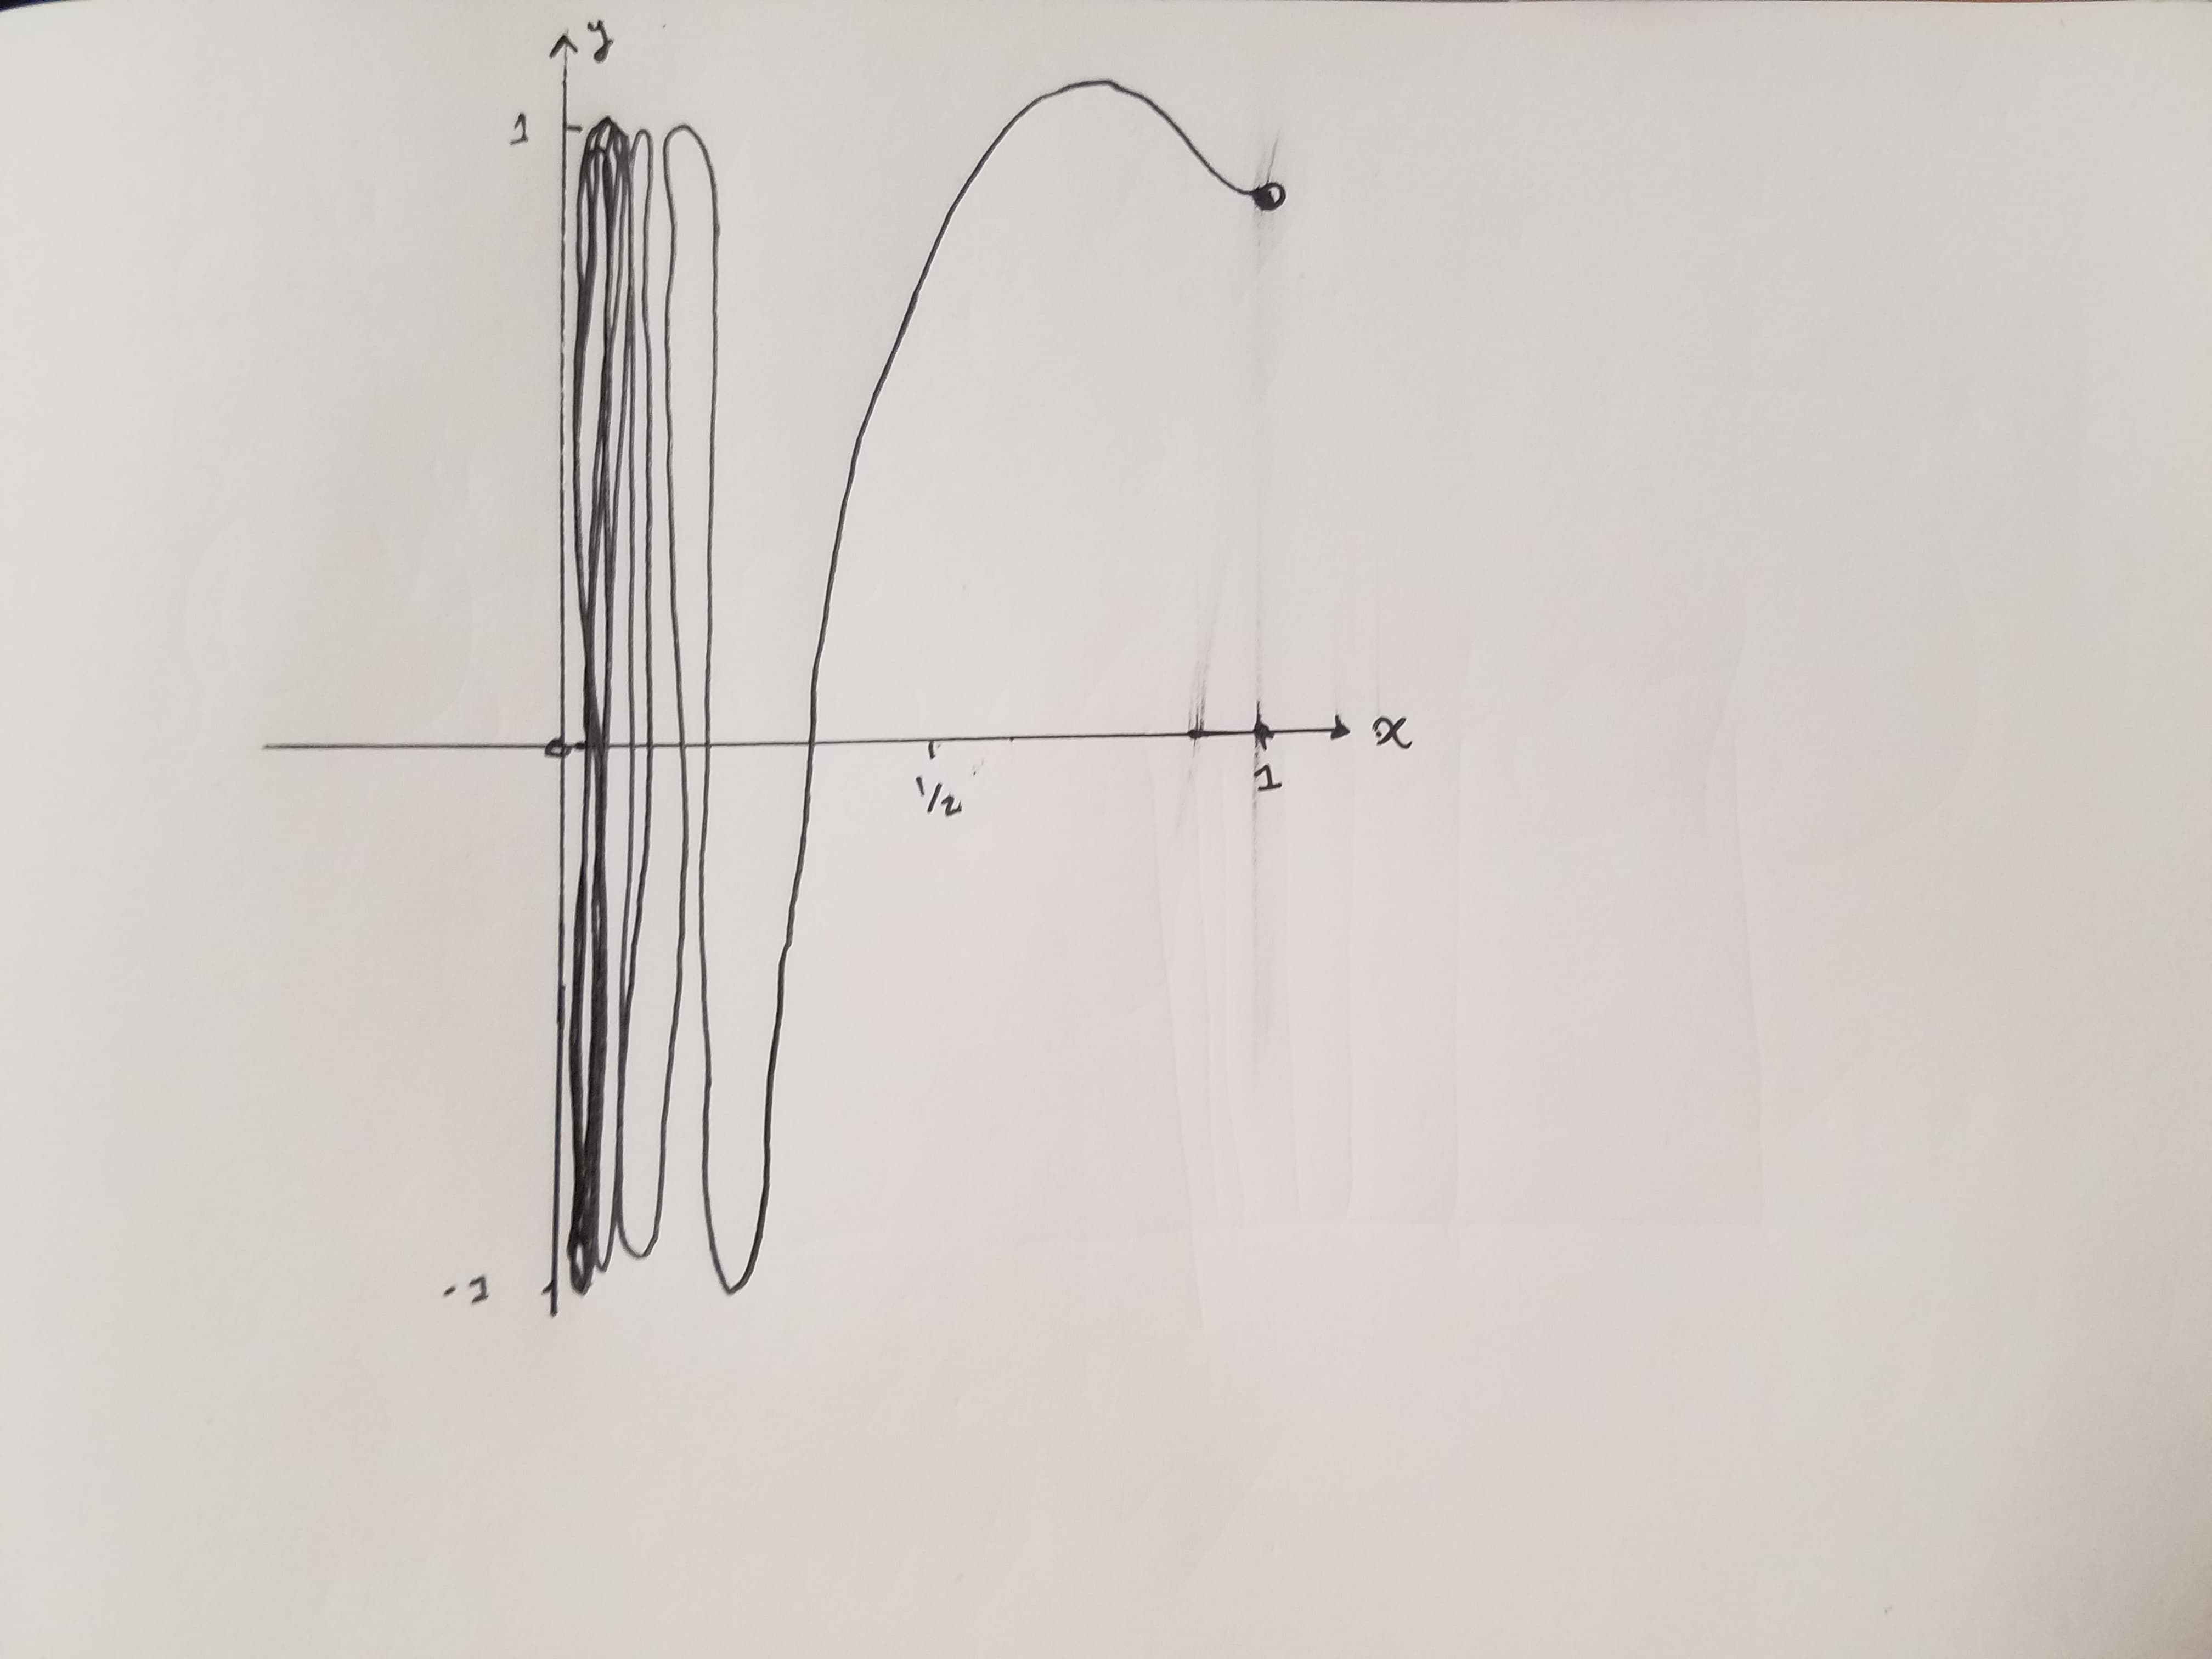
\includegraphics[width=0.5\textwidth]{topologist_sine_curve.jpg}
    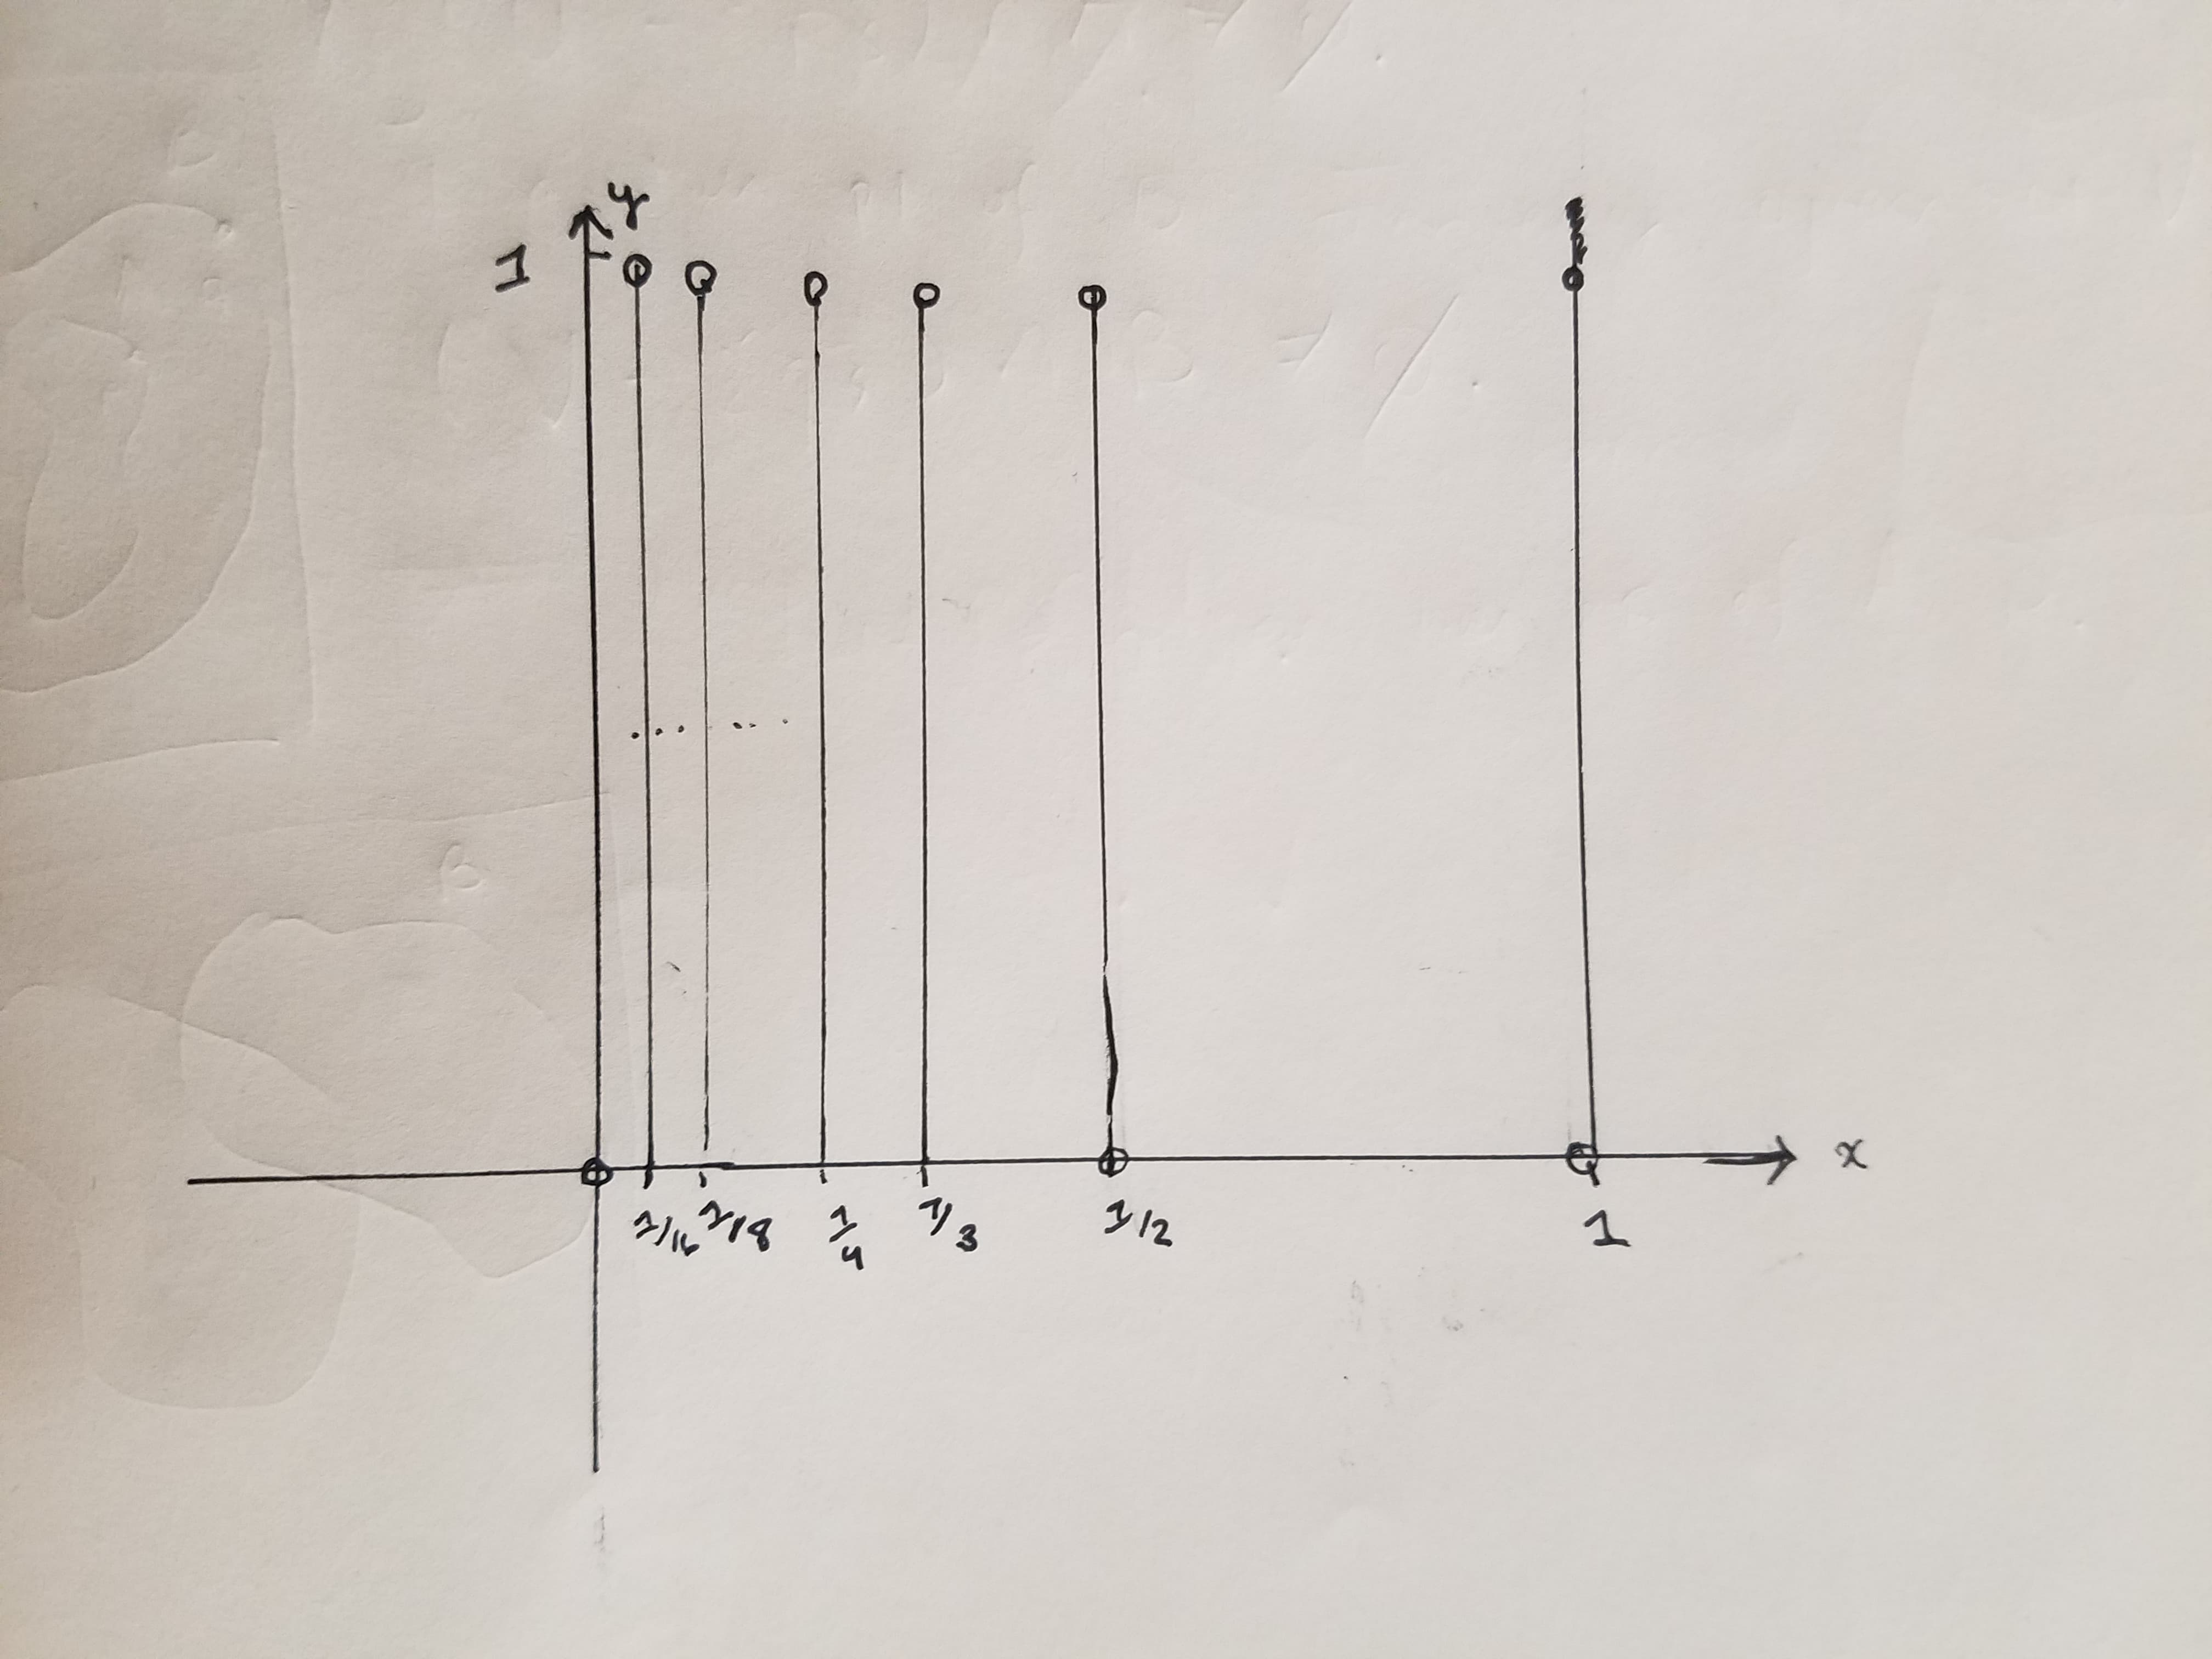
\includegraphics[width=0.5\textwidth]{topologist_comb.jpg}
    \caption{The lefthand drawing is the topologist's sine curve,
    while the right hand drawing is the topologist's comb.}
\end{figure}

\end{solution}

\begin{exercise}[Exercise 3.25]
    In the standard topology on $\mathbb{R}$, there
    exists a non-empty open subset $C$ of the closed unit interval $[0,
    1]$ that is closed, contains no non-empty open interval, and where no
    point of $C$ is an isolated point.
\end{exercise} 

\begin{solution}
    The rationals won't work because rationals aren't closed, since their
    limit points are irrationals. \\
    \\
    Consider the Cantor set. Everytime you try to construct an open
    interval it will eventually be able to escape and no longer be
    contained in the cantor set. It is closed because it contains an
    arbitrary intersection of closed sets.       
\end{solution}

\begin{problem}[Theorem 3.26] Let $A$ be a subset of a topological
    space $X$. Then $p$ is an interior point of $A$ if and only if
    there exists an open set $U$ with $p \in U \subset A$. 
\end{problem}

\begin{proof}
    First we start with the forward direction. Suppose that for some
    $p \in A$, there exsits an open set $U$ such that $p
    \in U \subset A$. Since $U$ is open and $U
    \subset A$, by definition we have that 
    $U \subset \text{Int}(A)$, and therefore $p \in
    \text{Int}(A).$ Thus $p$ must be an interior poiint. \\
    \\ 
    Now suppose that $p$ is an interior point of $A$. Then since $p
    \in \text{Int}(A) = \bigcup\limits_{U \subset A, U \in
    \mathscr{T}}U,$ we know that for at least one $U \in \mathscr{T}$,
    $p \in U \subset A$. Thus there exists an open set $U$ containing
    $p$ which is a subset of $A$, which is what we set out to show.
    With both directions proved, we have proved the theorem.
\end{proof}

\begin{exercise}[Exercise 3.27] 
    Show that a set $U$ is open in a topological
    space $X$ if and only if every point of $U$ is an interior point of
    $U$. 
\end{exercise}

\begin{solution}
We'll first prove the forward direciton. Let $U \subset X$, 
and suppose every point in $U$ is an
interior point of $U$. By Theorem 3.26 for all $p \in U$ 
there exists an
open set $V_p$ such that $p \in V_p \subset U.$ 
Since every point $p \in U$ is contained in an open ball
$V_p$ which is a subset of $U$, we have that $U$ must be an open 
set by Theorem 3.3.\\
\\
Now we prove the other direction. Suppose that $U$ is an open set.
Then by Theorem 3.3, for every point $p \in U$,
there exists an open ball $V_p$ such that $p \in V_p \subset U$.
But by Theorem 3.26, this means that every $p \in U$ is an
interior point of $U$, which is what we set out to show.

\end{solution}

\begin{problem}[Theorem 3.28] Let $A$ be a subset of a topological
    space $X$. Then $\text{Int}(A)$, $\text{Bd}(A)$ and
    $\text{Int}(X-A)$ are disjoint sets whose union equals $X$.
\end{problem}

\begin{proof}
    First we'll show that these sets are disjoint. Consider a point $p
    \in \text{Int}(A).$ By theorem 3.26, there exists an open
    ball $U$ of $p$ such that $p \in U \subset A$. Therefore,
    $p \notin \overline{X-A}$. This is because $p \notin (X-A)$, and
    $p$ is not a limit point of this set because not every open set of
    $p$ intersects with $X-A$. Namely, the open set $U \subset A$
    which we constructed earlier 
    contains $p$ but does not intersect $X-A$. Therefore $p \notin
    \overline{X-A}$. \\
    \\
    This fact helps us in two ways. Since $p \notin \overline{X-A}$,
    it is definitely true that $p \notin \text{Int}(X-A) \subset
    \overline{X - A}$, and that $p \notin \text{Bd}(A)$ since the
    definition of $\text{Bd}(A)$ is $\overline{A} \cap
    \overline{X-A}.$ Thus $\text{Int}(A)$ is disjoint with
    $\text{Bd}(A)$ and $\text{Int}(X-A).$ \\
    \\
    Finally we'll show that $\text{Int}(X-A)$ is disjoint with
    $\text{Bd}(A)$. Let $q \in \text{Int}(X-A)$. By Theorem 3.26 
    there exists an open set
    $U_q$ such that $q \in U_q \subset (X - A)$. Thus $q$ cannot be in
    $\overline{A}$. We can then conclude that $q \notin \text{Bd}(A)$
    because $\text{Bd}(A) = \overline{A} \cap \overline{X-A}$, and we
    just showed that $q \notin \overline{A}$. Therefore,
    $\text{Int}(X-A)$ is disjoint with $\text{Bd}(A)$. \\
    \\
    Now for the sake of contradiciton, suppose there exists a point $r
    \in X$ such that $r \notin \text{Int}(A) \cup \text{Bd}(A) \cup
    \text{Int}(X - A)$. Since $r \notin \text{Int}(A)$ and $r \notin
    \text{Int}(X - A)$, then by definition, we know that every open
    set containing $r$ must intersect $A$ and $X - A$. But this would
    imply that $r \in \text{Bd}(A)$, which is a contradiction. Thus
    there is no $r \in X$ such that $r \notin \text{Int}(A) \cup
    \text{Bd}(A) \cup \text{Int}(X - A)$, which means that $X =
    \text{Int}(A) \cup \text{Bd}(A) \cup \text{Int}(X - A)$.
\end{proof}

\noindent
\textbf{Exercise 3.29} 

\begin{exercise}[Exercise 3.29] 
    Pick several different subsets of $\mathbb{R}$,
    and for each one, finds its interior and boundary using:
    \begin{itemize}
        \item[1.] the discrete topology;
        \item[2.] the indiscrete topology;
        \item[3.] the finite complement topology;
        \item[4.] the standard topology.
    \end{itemize}
\end{exercise}

\begin{solution}
    \begin{itemize}
        \item[1.] Consider the set $(0,1).$ Since this is the discrete topology, we
        know that every subset of $\mathbb{R}$ is open. Therefore, the
        interior of $(0,1)$ is simply itself. The boundary of this set is
        simply empty, since $\overline{(0,1)} \cap \overline{R-(0,1)} =
        \emptyset.$
    
        \item[2.] For $(0,1)$, the interior is $\emptyset$, since the empty set is
        the largest set contained in $(0,1)$. On the other hand, the boundary
        is simply the set $\{0, 1\}$ since $(0,1) \cap \mathbb{R} - (0,1) =
        \{0,1\}.$ 
    
        \item[3.] On the finie complement topology, $(0,1)$ does not have an
        interior. This is because on this topology there does not exist an
        open set contained in $(0,1)$. The set is also not closed, since it
        does not contain its limit points. In fact, every point in
        $\mathbb{R}$ is a limit point of the set, so $\overline{(0,1)} =
        \mathbb{R}$ and $\overline{\mathbb{R} - (0,1)} = \mathbb{R}$, so the
        boundary is simply $\mathbb{R}$.
    
        \item[4.] For the standard topology, the interior is simply $(0,1)$. The
        boundary is $\{0, 1\}$, since $\overline{(0,1)} \cap
        \overline{\mathbb{R} - (0,1)} = \{0,1\}.$
    \end{itemize}
\end{solution}

\begin{problem}[Theorem 3.30] Let $A$ be a subset of the topological
    space $X$ and let $p$ be a point in $X$. If $\{x_i\}_{i \in
    \mathbb{N}} \subset A$ and $x_i \rightarrow p$, then $p$ is in the
    closure of $A$.
\end{problem}

\begin{proof}
    Since $x_i \rightarrow p$, we know that for every open set $U$
    containing $p$, there exists an $N \in \mathbb{N}$ such that $x_i
    \in U$ for $i > N$. However, for all $n \in \mathbb{N}$, we know
    that $x_n \in A$. Therefore, we know that $(U-\{p\}) \cap A \ne
    \emptyset$ for any open set $U$ containing $p$. Thus $p$ must be a
    limit point of $A$, so $p$ is in the closure of $A$.

    \begin{figure}[h!]
        \centering
        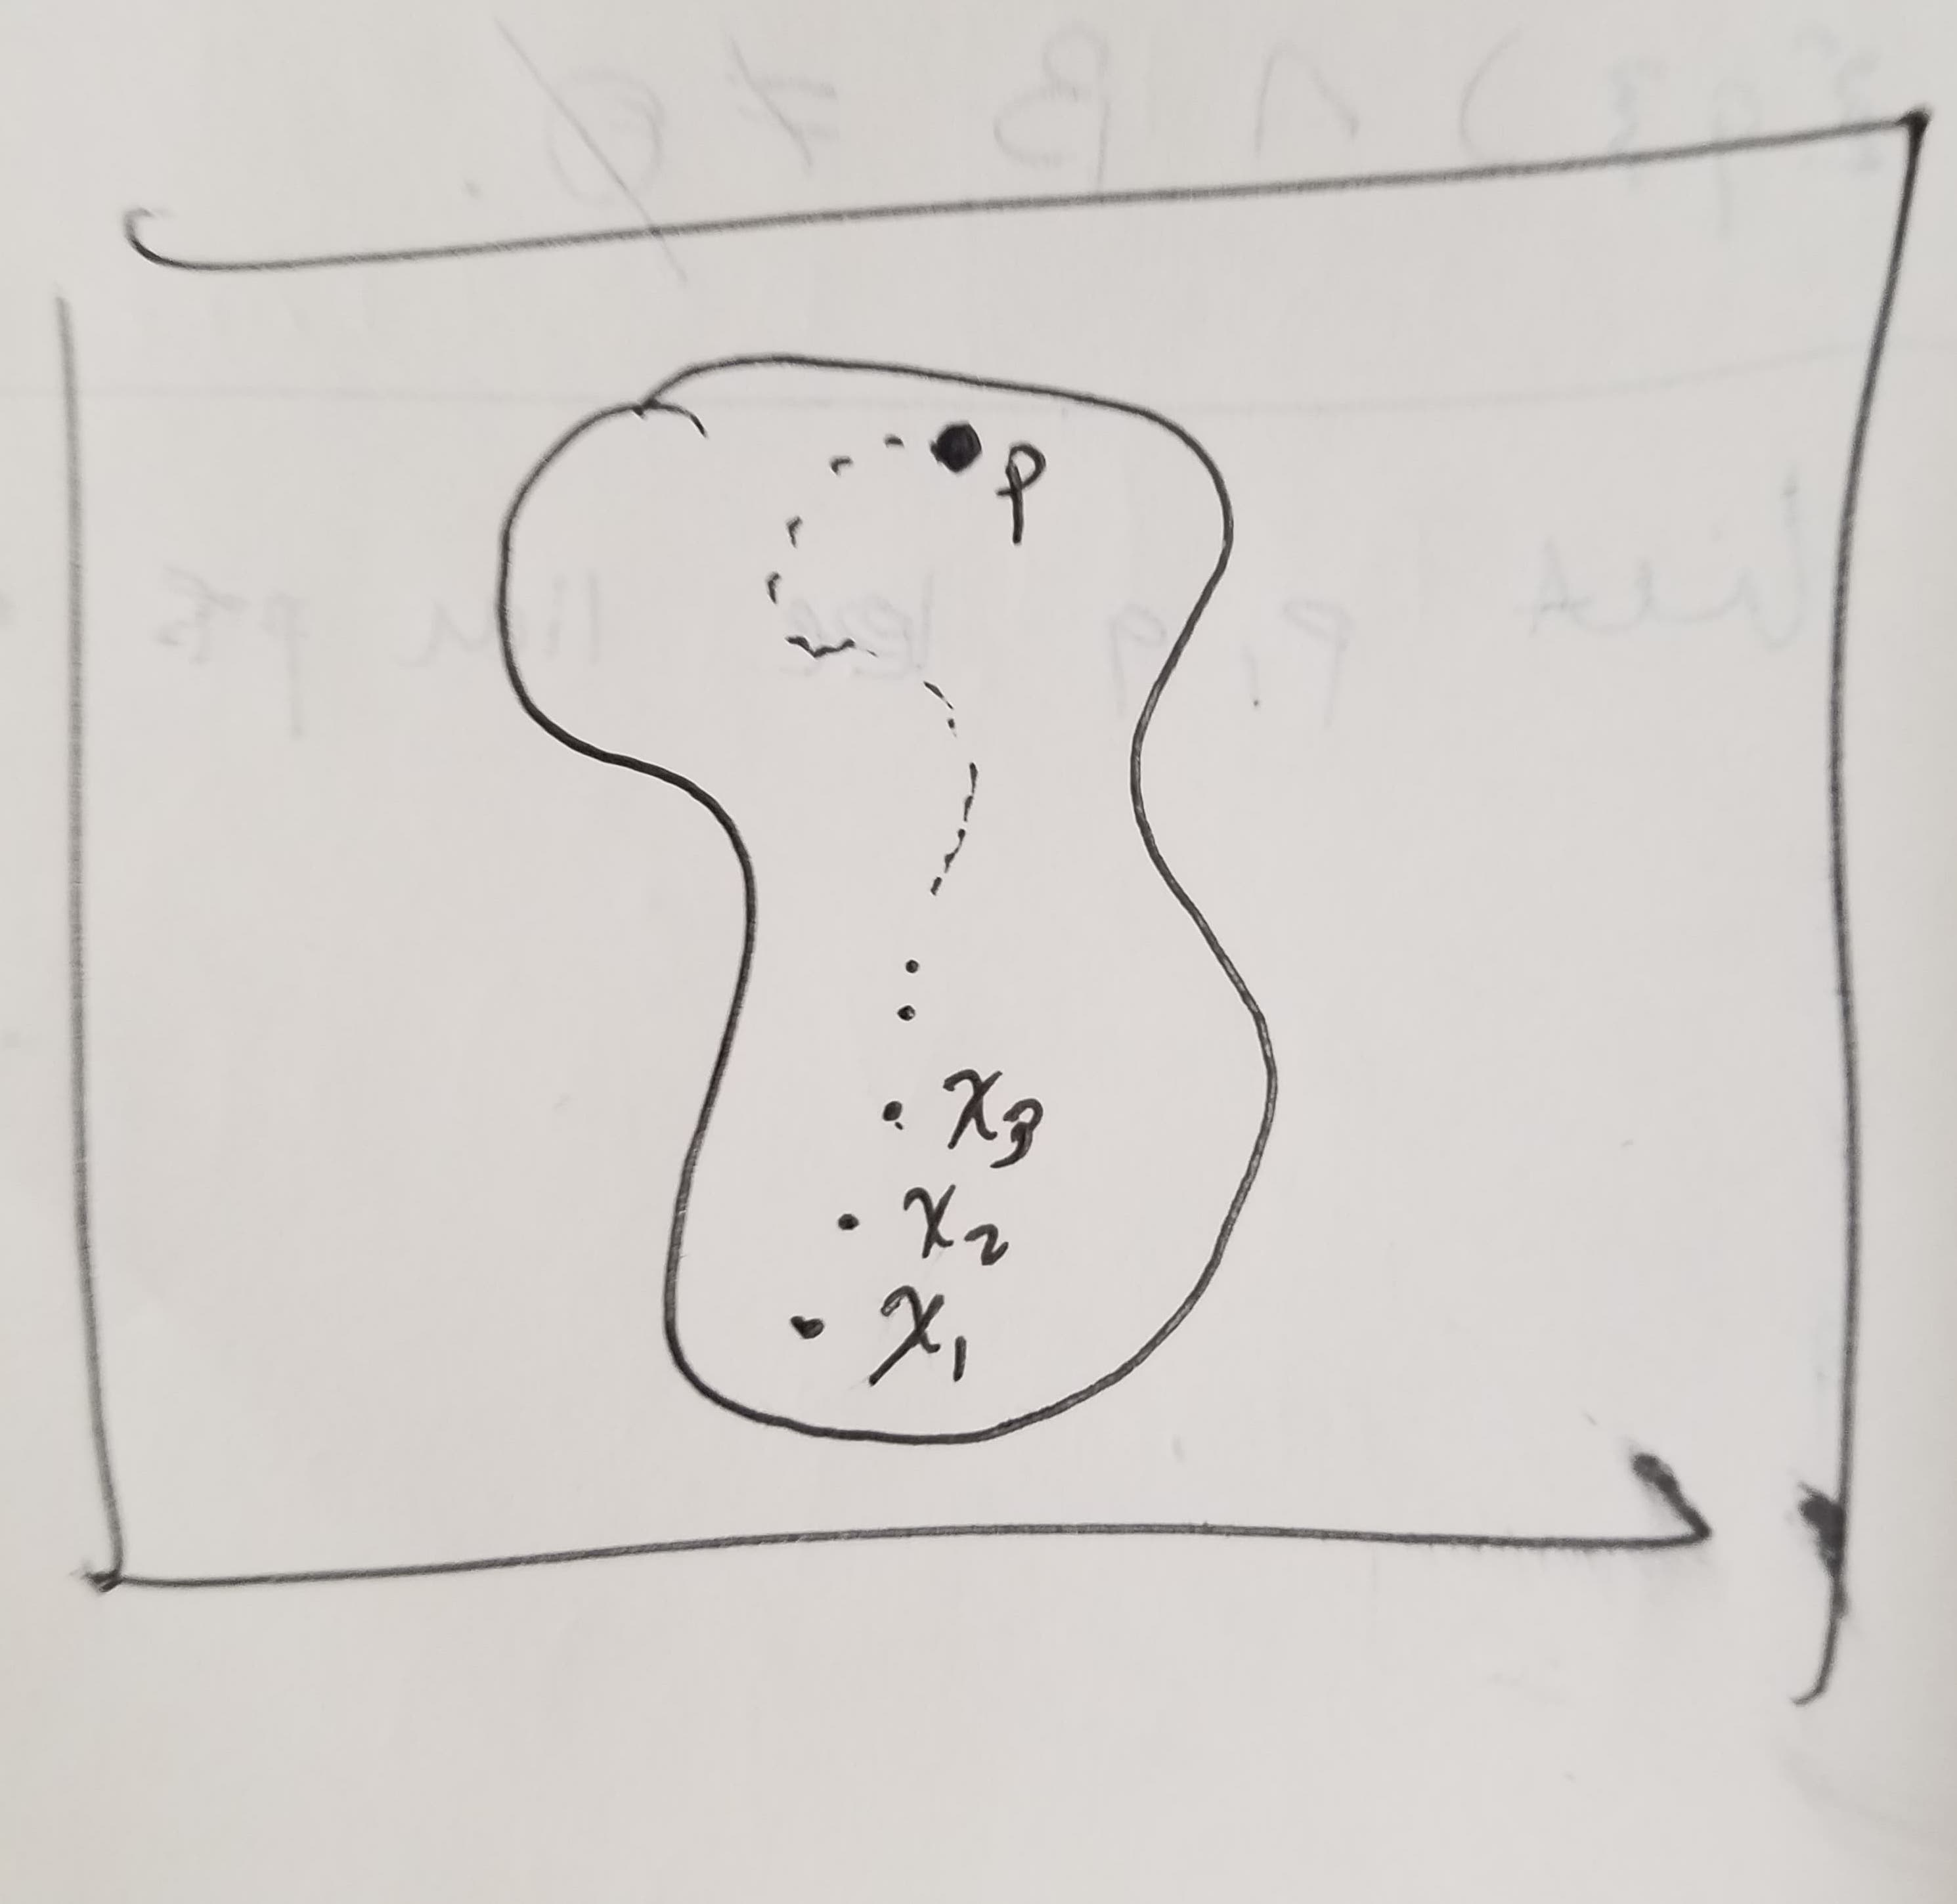
\includegraphics[width=0.5\textwidth]{sketch_theorem_3_30.jpg}
        \caption{With the drawing, its easy to see that if all the points
        in the sequence must be in $A$, then the limit of the sequence is
        at most in the closure of $A$.}
    \end{figure}
\end{proof}

\begin{problem}[Theorem 3.31] In the standard topology on
    $\mathbb{R}^n$, if $p$ is a limit point of a set $A$, then there
    is a sequence of points in $A$ that converge to $p$.
\end{problem}

\begin{proof}
    Since $p$ is a limit point of $A$, we know that for every open set
    $U$ containing $p$, we have that $(U - \{p\}) \cap A \ne
    \emptyset$. Thus let $\epsilon > 0$, and consider the sequence of
    balls $B(p, \epsilon/n)$ containing $p$ of radius $\epsilon/n$.
    Then since $(B(p, \epsilon/n) - \{p\}) \cap U \ne \emptyset$, for
    each $n$ there must exist a $q \in A$ such that $q \in (B(p,
    \epsilon/n) - \{p\})$. Label these such $q$ as $q_n$. \\
    \\
    Now let $\delta > 0$, and consider the open ball $B(p, \delta)$.
    Then there exists an $m \in \mathbb{N}$ such that $\epsilon/m <
    \delta$ so that $B(p, \epsilon/m) \subset B(p, \delta).$ In other
    words, for any open set $U$ about $p$, there exists a number $m
    \in \mathbb{N}$ such that for all $n > m$, $q_n \in U$. Therefore
    we can conclude that $\{q_n\}$ is a sequence of points where for
    all $n \in \mathbb{N}$, $q_n \in A$ and $q_n \rightarrow p$, which
    is what we set out to show. \\
    \\
    In general, the limit point of a set is not the same thing as the
    limit of a sequence.
\end{proof}

\begin{exercise}[Exercise 3.32]
    Find an example of a topological space and a convergent sequence in
    that space, where the limit of the sequence is not unique.
\end{exercise}

\begin{solution}
An easy example can be found with the indiscrete topology on
$\mathbb{R}$. Consider the sequence $1, 2, 3, \dots$. Then every $x
\in \mathbb{R}$ is a limit of the sequence, since the only open set
containing any point is $\mathbb{R}$ which obviously contains every
point of the sequence. 
\end{solution}

\begin{exercise}[Exercise 3.33]
    1. Consider sequences in $\mathbb{R}$ with the finite complement
    topology. Which sequences converge? To what value(s) do they
    converge?\\
    2. Consider sequences in $\mathbb{R}$ with the countable complement
    topology. Which sequences converge? To what value(s) do they
    converge?
\end{exercise}

\begin{solution}
Consider the sequence $\left\{\dfrac{1}{n} | n \in \mathbb{R}\right\}$ and
$\left\{\dfrac{n}{n+1} | n \in \mathbb{N}\right\}.$ Then on the finite complement
topology, we see that both sequences are convergent. This is because,
for either of the sequences, we cannot construct an open set around a
limit point which does not include points of the sequence, since every
open set is of the form $\mathbb{R} - X$, where $X$ is a finite set,
and both sequences are countably infinite. In addition, the
convergence of both sets is not unique, since on this topology, every
open set of any $x \in \mathbb{R}$ will inevitably include points of
the sequences. \\
\\
In both cases, neither of the sequences are convergent. This is
because for any $x \in \mathbb{R}$ which could be a limit point of the
sequence, we can construct an open set $U$ containing $x$ where $U =
\mathbb{R} - \left\{\dfrac{1}{n} | n \in \mathbb{R}\right\}$. Thus by the
definition of a limit of a sequence, neither of these points converge.
\\
Note: what is the relationship between the sequences which are and
aren't convergent on these two different topological spaces? It seems
like a finite sequence wouldn't be convergent on the finite complement
topology, while a infinite one is, and that an infinite sequence isn't
convergent on the countable complement topology, while a finite one
is. 

\end{solution}

\end{document}
